\chapter{Core JS}
\label{core-js}
\paragraph{} Javascript is the final distinct language that we'll study and makes up the third part of our triumvirate of core Web technologies alongside HTML and CSS.
\paragraph{} Assuming that HTML enables us to define information, and CSS enables us to style that information visually, it is JavaScript that enables us to dynamically interact with our information, to manipulate our pages, or even to create and alter them on the fly (as well as to do other cool stuff like implement games, graphics, sound, etc.). Javascript is a full blown programming language that just happens to live, mostly, in the web browser. In this unit we'll introduce ourselves to the core of the language.

\section{JavaScript}
\paragraph{} JavaScript (JS) is the third part of our triumvirate of web technologies alongside HTML and CSS. Just as HTML and CSS enable us to delineate content from presentation, JS enables us to further separate out functionality and behaviour from a Web page’s content and presentation.

\paragraph{} So what is JavaScript? It is a general purpose programming language, more specifically a high-level, dynamic, weakly typed, prototype-based, multi-paradigm, interpreted programming language. 

\paragraph{} For our purposes in WebTech, focussing on the client-side user interface, it is a browser hosted programming language. This means that JavaScript code runs inside the browser. JavaScript was originally a project at Netscape which lead to the first Javascript implementation. This was then formalised to produce the ECMAScript specification. Whilst the actual name ``Javascript'' is a trademark of Oracle, anyone can implement the specification to produce their own version of the language. As a result there is no single Javascript implementation, Instead there are a range of different engines in most web browsers. Each implements the ECMAScript specification to varying degrees so some features might be missing and some engines have additional features. This means that Web developed using JavaScript can be complex.


\section{JS The Language}
\paragraph{} JS is multi-paradigm -- This means that it can support a range of different programming styles, for example, event-driven, functional, imperative, and Object Oriented. This means that it is very flexible and adaptable to fit a wide range of problems and enables you to approach a solution driven by the needs of the problem domain rather than the needs of the language.
\paragraph{} In addition to the core language, which we'll investigate very soon, JS provides an API for common tasks such as working with text, arrays of dates, dates, regular expressions, as well as Web specific APIs for doing DOM manipulation.
\paragraph{} Note that there is no core language support for direct input/output (I/O) like we'd expect in most languages. This is because the host environment, the browser provides the "place" where your code runs, so the host environment provides the ability to do input and output. Input data usually comes from the browser, usually related to the web page that is loaded at any given time. Output is also handled by the browser, usually either through updates or manipulations to the currently loaded web page, calls to remote APIs over the network, or through browser logging mechanisms.
\paragraph{} In most languages we'd expect I/O as well as other facilities like networking, storage, and graphics to be part of the standard library of facilities. In JS these are provided either by the host environment, i.e. the browser API or through additional libraries and APIs.
\paragraph{} It's worth considering JS as a kind of ``glue language''. It is meant to be easy for everyone from web designers and part-time programmers as well as hobbyists to assemble the components of web pages to create their sites.


\section{An Aside: Java(Script)?}
\paragraph{} If you're confused and are wondering about the naming of Javascript and Java, that's entirely understandable. These are two wholly separate languages so you shouldn't confuse one for the other. Whilst they might share some syntax or have similar libraries, and overlapping names, these are merely superficial similarities.
\paragraph{} Brendan Eich was originally employed by Netscape to write a version of the Lisp variant Scheme to run in the browser. This was originally meant to fulfil the requirements that JS now fulfils. However the Netscape management made the decision that Javascript should “look like Java” which was the hot new thing in the mid to late 1990s. So a Java-like, or Java-inspired language, called JavaScript, was developed and released in Netscape's browser. The rest is, as they say, history.


\section{JS Engines}
\paragraph{} We've already established that JS is interpreted, Virtual Machine (VM) based, and runs within a host environment. In this context interpreted means that JS source-code is read, line by line, and the computer decides, on-the-fly, what to do as a result. This should be contrasted with languages like C in which the source-code is compiled into a different form before execution. VM based means that rather than running directly on the host machine, JS is run within a special execution environment which does the job of interpreting the source-code and working out what to do, then doing it. All languages run within a host environment but usually this just refers to the hardware platform and the operating system. However, in the case of JS running on the Web, the host environment is the web browser or whichever other, JS enables user agent is executing the JS.
\paragraph{} Because browsers do more than merely execute JS, the part of the browser, the JS VM, that interprets and executes JS source-code is often called the JS engine. There are many JS engines,  and as we pointed out earlier, you can implement your own from the JS specification, but some implementations are more important than others usually because they are widely used or have particularly good performance characteristics. These engines include:

\begin{description}
\item [V8] The Google Chrome JS engine. Note that V8 is also used in Node.js, another technology that enables JS code to be run outside of the browser host environment.
\item [Spidermonkey] The Firefox JS engine.
\item [JavaScriptCore] This is marketed as ``Nitro'' and is the JS engine used in Safari on MacOS platforms.
\end{description}

\paragraph{} You can work with JS in the browser fairly easily as you would expect. But you can also install a standalone tool to run JS outside the browser (e.g. Node.js) — this enables Javascript to run server side. For some people, using a similar implementation language for code that runs in the browser and code that runs on the server, for server-side dynamic sites, is an attractive prospect. Note though that whilst there are limited options for languages that run directly in the browser, most languages can be used to create server-side functionality.



\section{What is JavaScript for?}
\paragraph{} JS is a, slightly weird, general purpose programming language. This means that we aren't limited to just web-oriented programming tasks. Basically any programming task that you could want to solve using any other language, can also be solved in JS.
\paragraph{} However Web programming is the \emph{raison d'$\hat{e}$tre} for JS. This means, primarily, interacting with the DOM for a given web page and also interacting with the user agent. By interacting with the DOM we mean that we can use JS to alter or replace any HTML element for the page loaded in the current browser tab or even to completely discard the current content and replace it with a new page entirely generated from JS. There are lots of API functions in JS that support manipulating the DOM in a variety of ways. By interacting with the user agent, we mean that we can use JS to manipulate the host environment provided by the browser. Most browsers provide a set of APIs or Application Programming Interfaces that support audio, graphics, client-side data storage and a wealth of other functionality.
\paragraph{} We said primarily above. A secondary use of JS is to provide a server-side environment so that our core tools can be (reasonably) cohesive whether they are operating on the server-side or the client-side. Finally, a tertiary use of JS is as a general purpose scripting language where any other scripting language might be used but this is a much more minority pursuit.



\section{What Does JS look like?}
\paragraph{} On its own JS looks like this:

\begin{lstlisting}
	console.log("hello world");
\end{lstlisting}

\paragraph{} You can try that out by typing it into the JS console in your browser. This just executes any JS that you type in immediately in the style of a Read-Evaluate-Print-Loop (REPL) and is a useful way to play around with JS as you are learning the language.

\paragraph{} Realistically though you are more likely to see JS in the context of a web page. Here is one example:

\begin{lstlisting}
<!DOCTYPE html>
<html>
	<head>
    		<title>Example</title>
  	</head>
  	<body>
    		<button id="hellobutton">Hello</button>
    		<script>
        document.getElementById('hellobutton').onclick = function() {
            alert('Hello world!');     
            var myTextNode = document.createTextNode('Some new words.');
            document.body.appendChild(myTextNode);   
        };
    		</script>
  	</body>
</html>
\end{lstlisting}

\paragraph{} In this case the JS is hosted within our HTML document between <script> tags. Usually we would actually store our JS outside the HTML and reference the JS source file in the same way that we stores CSS in external files. But for our first exposure to JS it is easier to use a single mixed example. You can type the code above into an html file, save it as hellojs.html and then open it in your browser. Note that in the document we are creating an HTML button element and giving it an ID. We are then creating some JS that provides a function that runs when the button is clicked. We use the buttons ID to identify it from other HTML elements, although there are no others in this example. We use a DOM API function to access the button element by supplying the ID to the document.getElementById function. Once we have a reference to the button element we are then attaching a function to it which first creates a popup alert box saying ``Hello world!'' and then we're creating a new element, a text node, setting the content of the text node to ``Some new words.'' and then appending the new text node to the HTML document displayed in the browser so that the content of the page is changed by our JS. 


\section{Using Javascript}
\paragraph{} Similar to CSS, and as noted above, we have three basic choices for how to integrate our HTML with our JS. These options are inline, in a script block, and in an external script file.

\paragraph{} Inline looks like this:

\begin{lstlisting}
<button id="hellobutton" onclick="alert('Hello World')">Click Me</button>
\end{lstlisting}

\paragraph{} Basically we are directly inserting the JS into the element to which we want it to apply. Useful in some contexts but having all of the same drawbacks that we explored earlier when applying style directly inline onto HTML elements.

\paragraph{} We can also use JS within a script block, e.g. a pair of <script></script> in our HTML page.

\begin{lstlisting}
<script>
    document.getElementById('hellobutton').onclick = function() {
        alert('Hello world');
    };
</script>
\end{lstlisting}


\paragraph{} We can also use an external script. In this case we need to tell the HTML document where to find any associated JS. We do that by placing a <script> tag into either the <head> or the <body> of the HTML file. There are some differences in how this is done between versions of HTML though.

\paragraph{} HTML 4

\begin{lstlisting}
	<script type="text/javascript" src=“javascript.js"></script>
\end{lstlisting}

\paragraph{} HTML 5
\begin{lstlisting}
	<script src="javascript.js"></script>
\end{lstlisting}

\paragraph{} Note that practically speaking you can use any number of external scripts and reference them from your HTML page. This means that you have significant flexibility in organising your JS code into separate files.



\section{JS in the Browser Console}
\paragraph{} As we saw earlier, we can execute JS in the browser's console. This is useful for learning JS and experimenting without the hassle of setting up an HTML file to host it. However we’ll quickly grow beyond this approach. Note though that the browser console does give us a small programming environment almost anywhere where there is a reasonably modern web browser. This is very useful to be aware of and we'll make the most of it for the next few examples.
\paragraph{} Let's look at some simple examples of how we can write JS directly in the browser console. I encourage you to try them out yourself, and then to use the functionality in each as a starting place for exploring the JS language API and for your own learning experiments.


\section{Hello Napier}
\paragraph{} This is basically the example we saw a few moments ago, but now with added screenshot goodness. We've included it as some form of "Hello World" program as is the traditional starting place for most new programming exercises.

\begin{figure}[H]
\centering
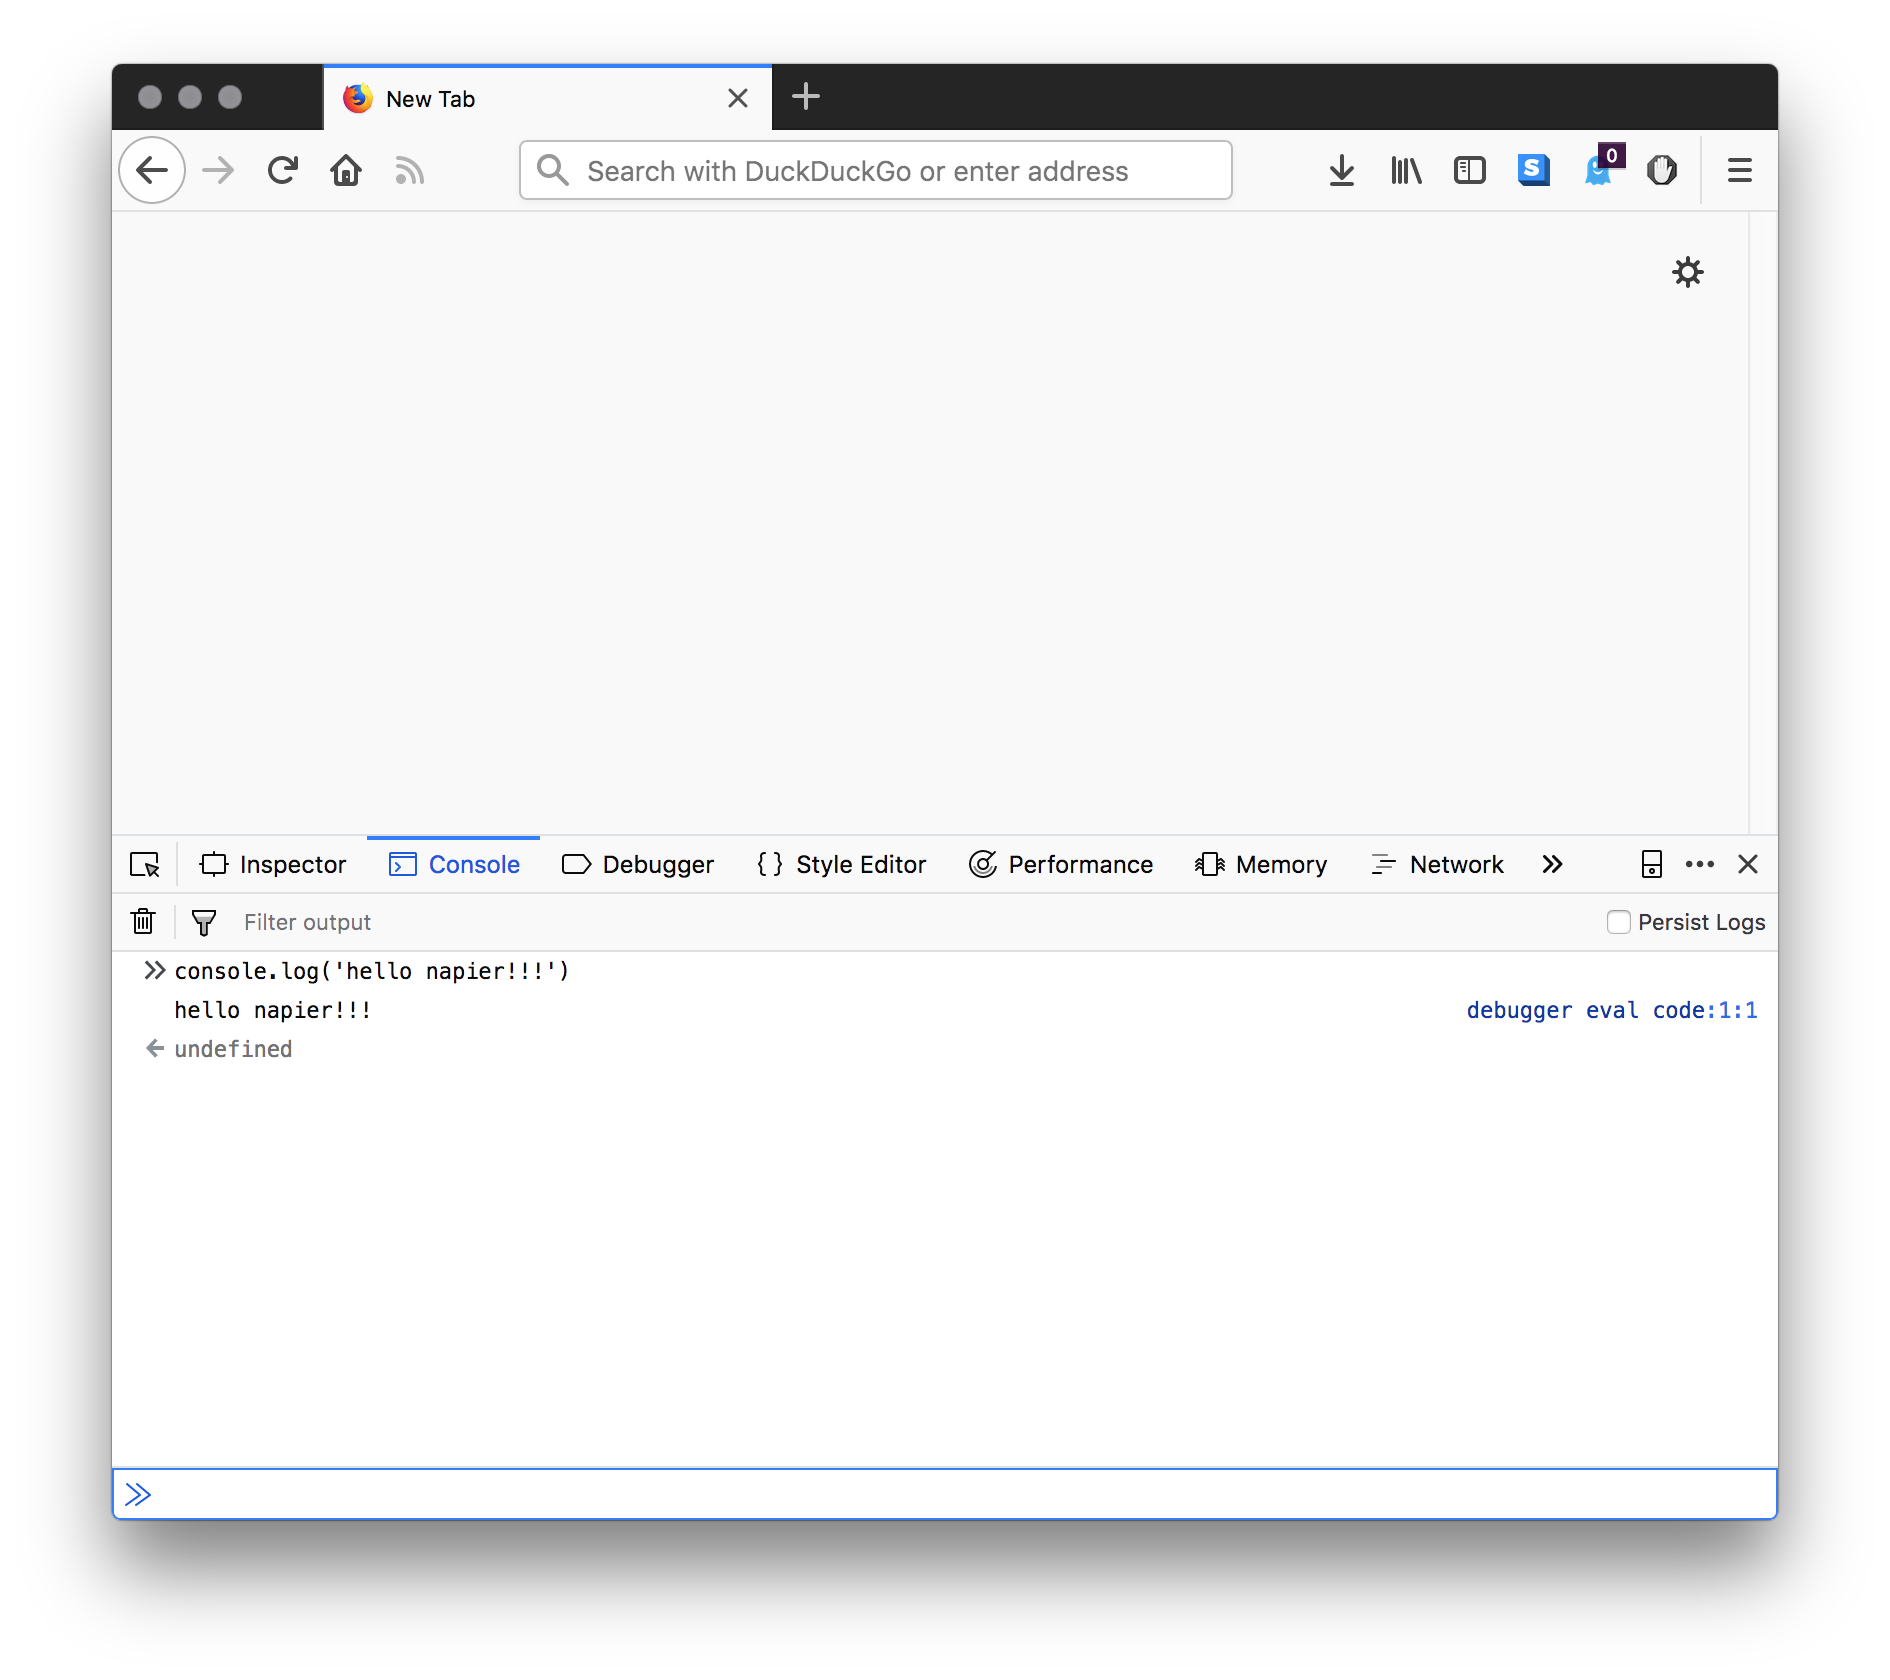
\includegraphics[width=0.8\textwidth]{figures/hello-napier}
\label{fig:hello-napier}
\caption{}
\end{figure}


\section{Interact with the Web Page/Screen}
\paragraph{} In this example we use the browser DOM manipulation API to access the background colour setting of the document body so that we can alter it to a different colour. This basic approach works for many of the style elements provided by CSS to enable us to programmatically manipulate a page's style.

\begin{figure}[H]
\centering
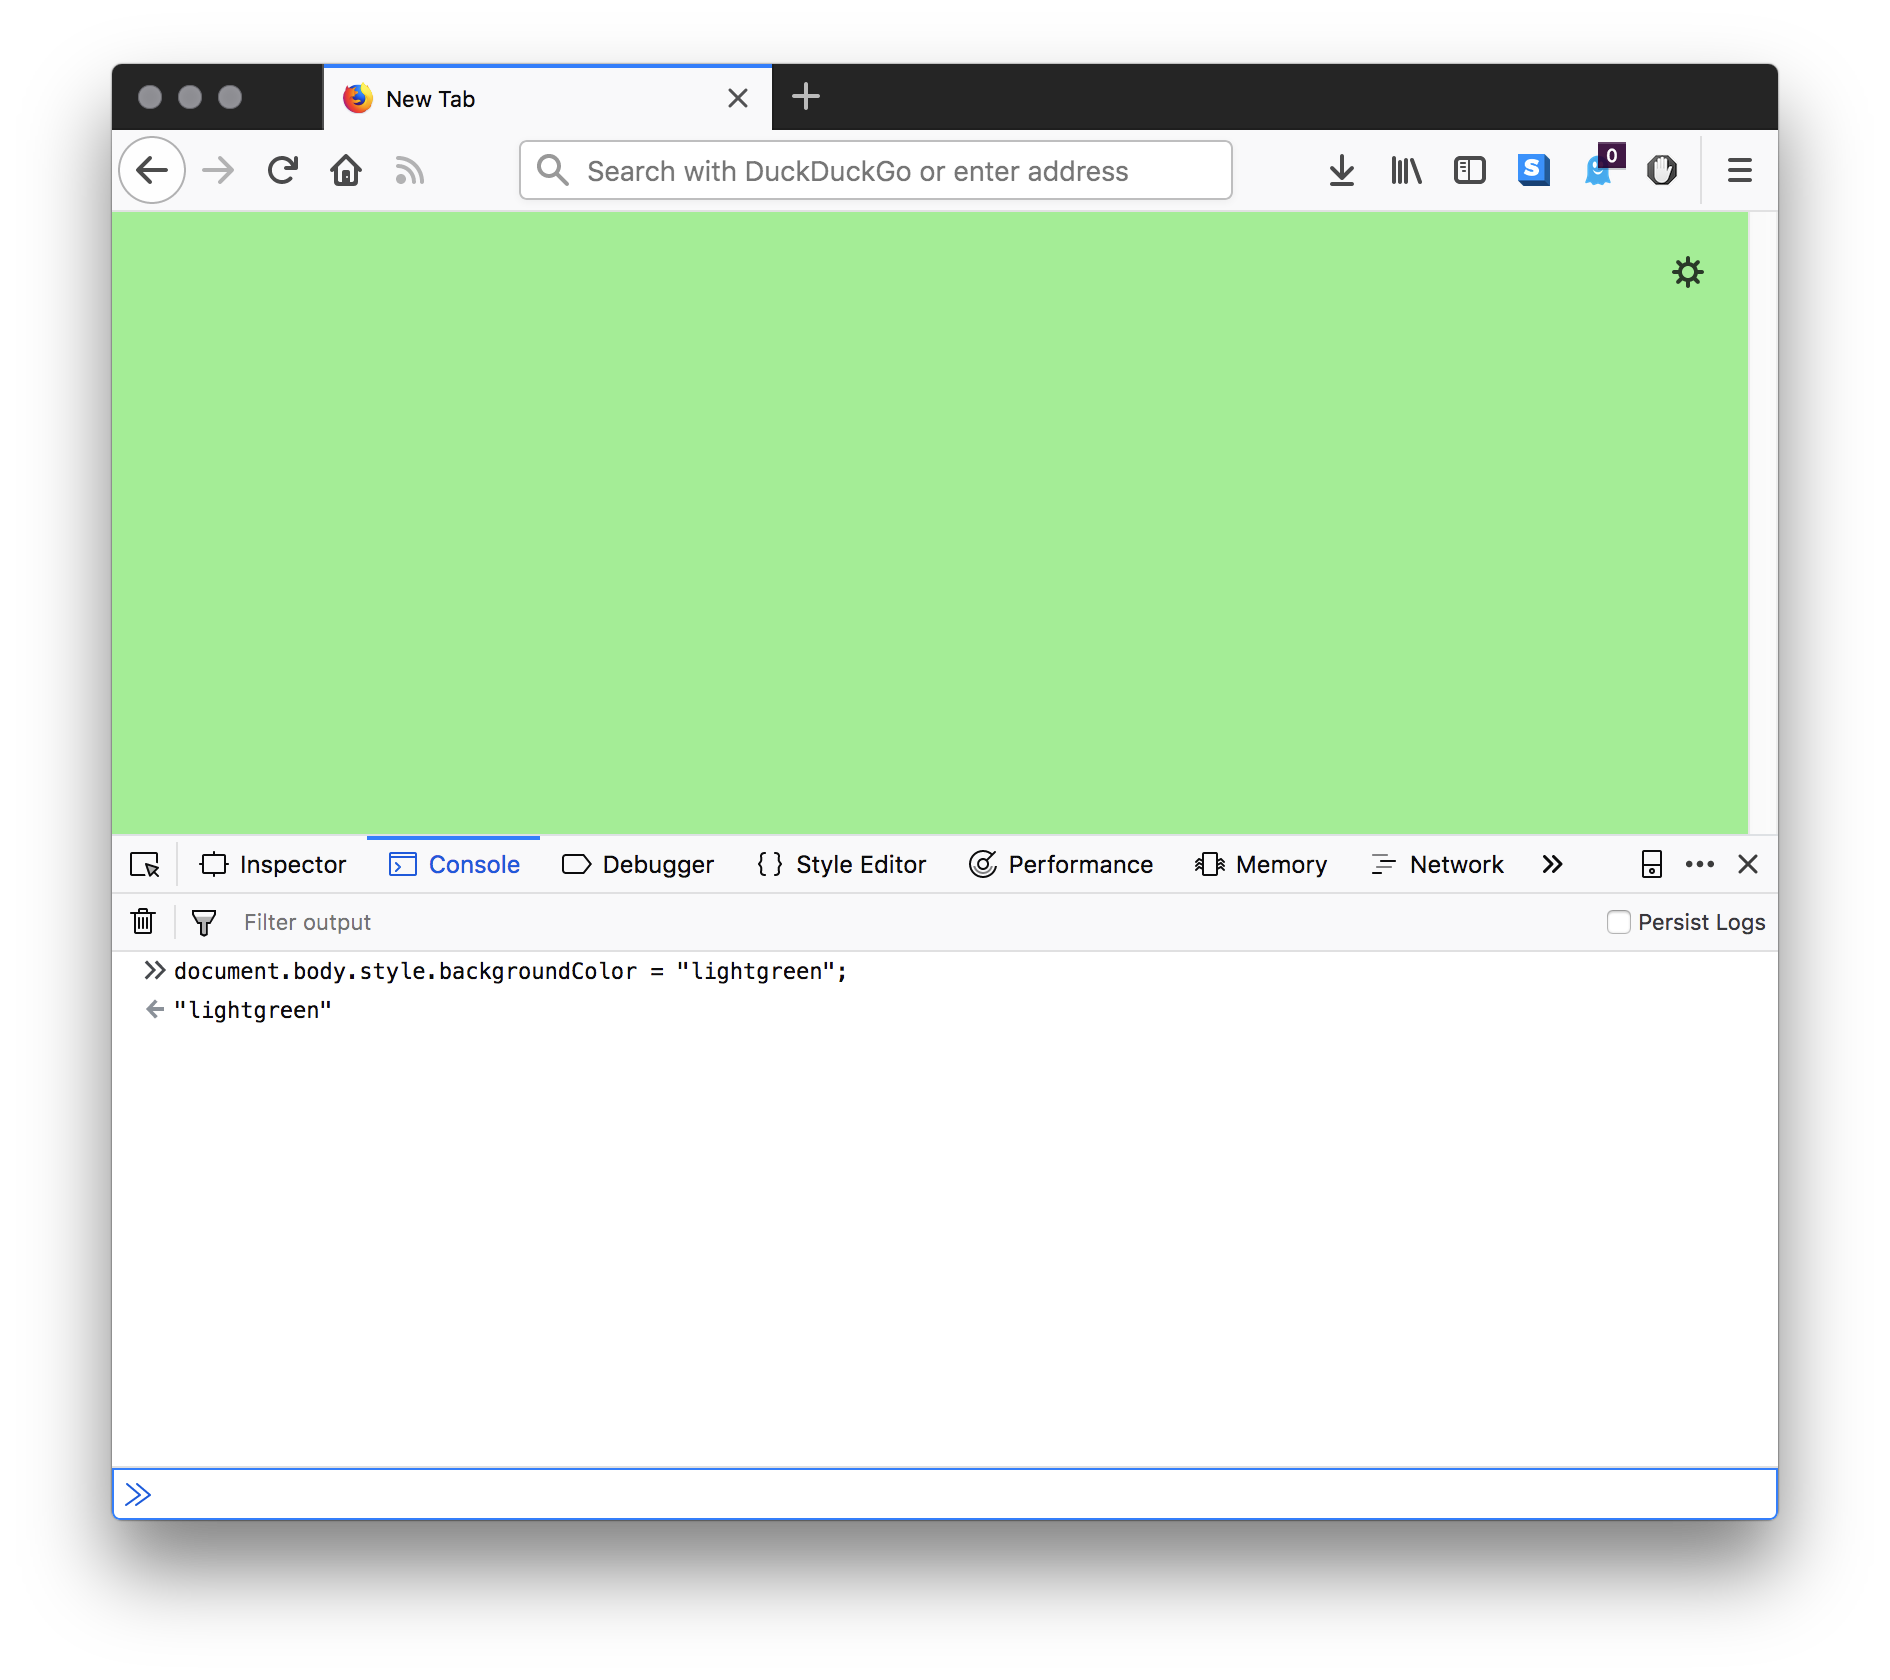
\includegraphics[width=0.8\textwidth]{figures/js-screen-interaction}
\label{fig:js-screen-interaction}
\caption{}
\end{figure}


\section{Use standard JavaScript functions}
\paragraph{} We can use JS language functions to provide information which can then be displayed on the current web page. In this example we create a new variable, called 'd' and then assign it the value returned by the built-in Date function. We then replace the HTML content of the current document displayed in the web browser to include the value stored in our variable.

\begin{figure}[H]
\centering
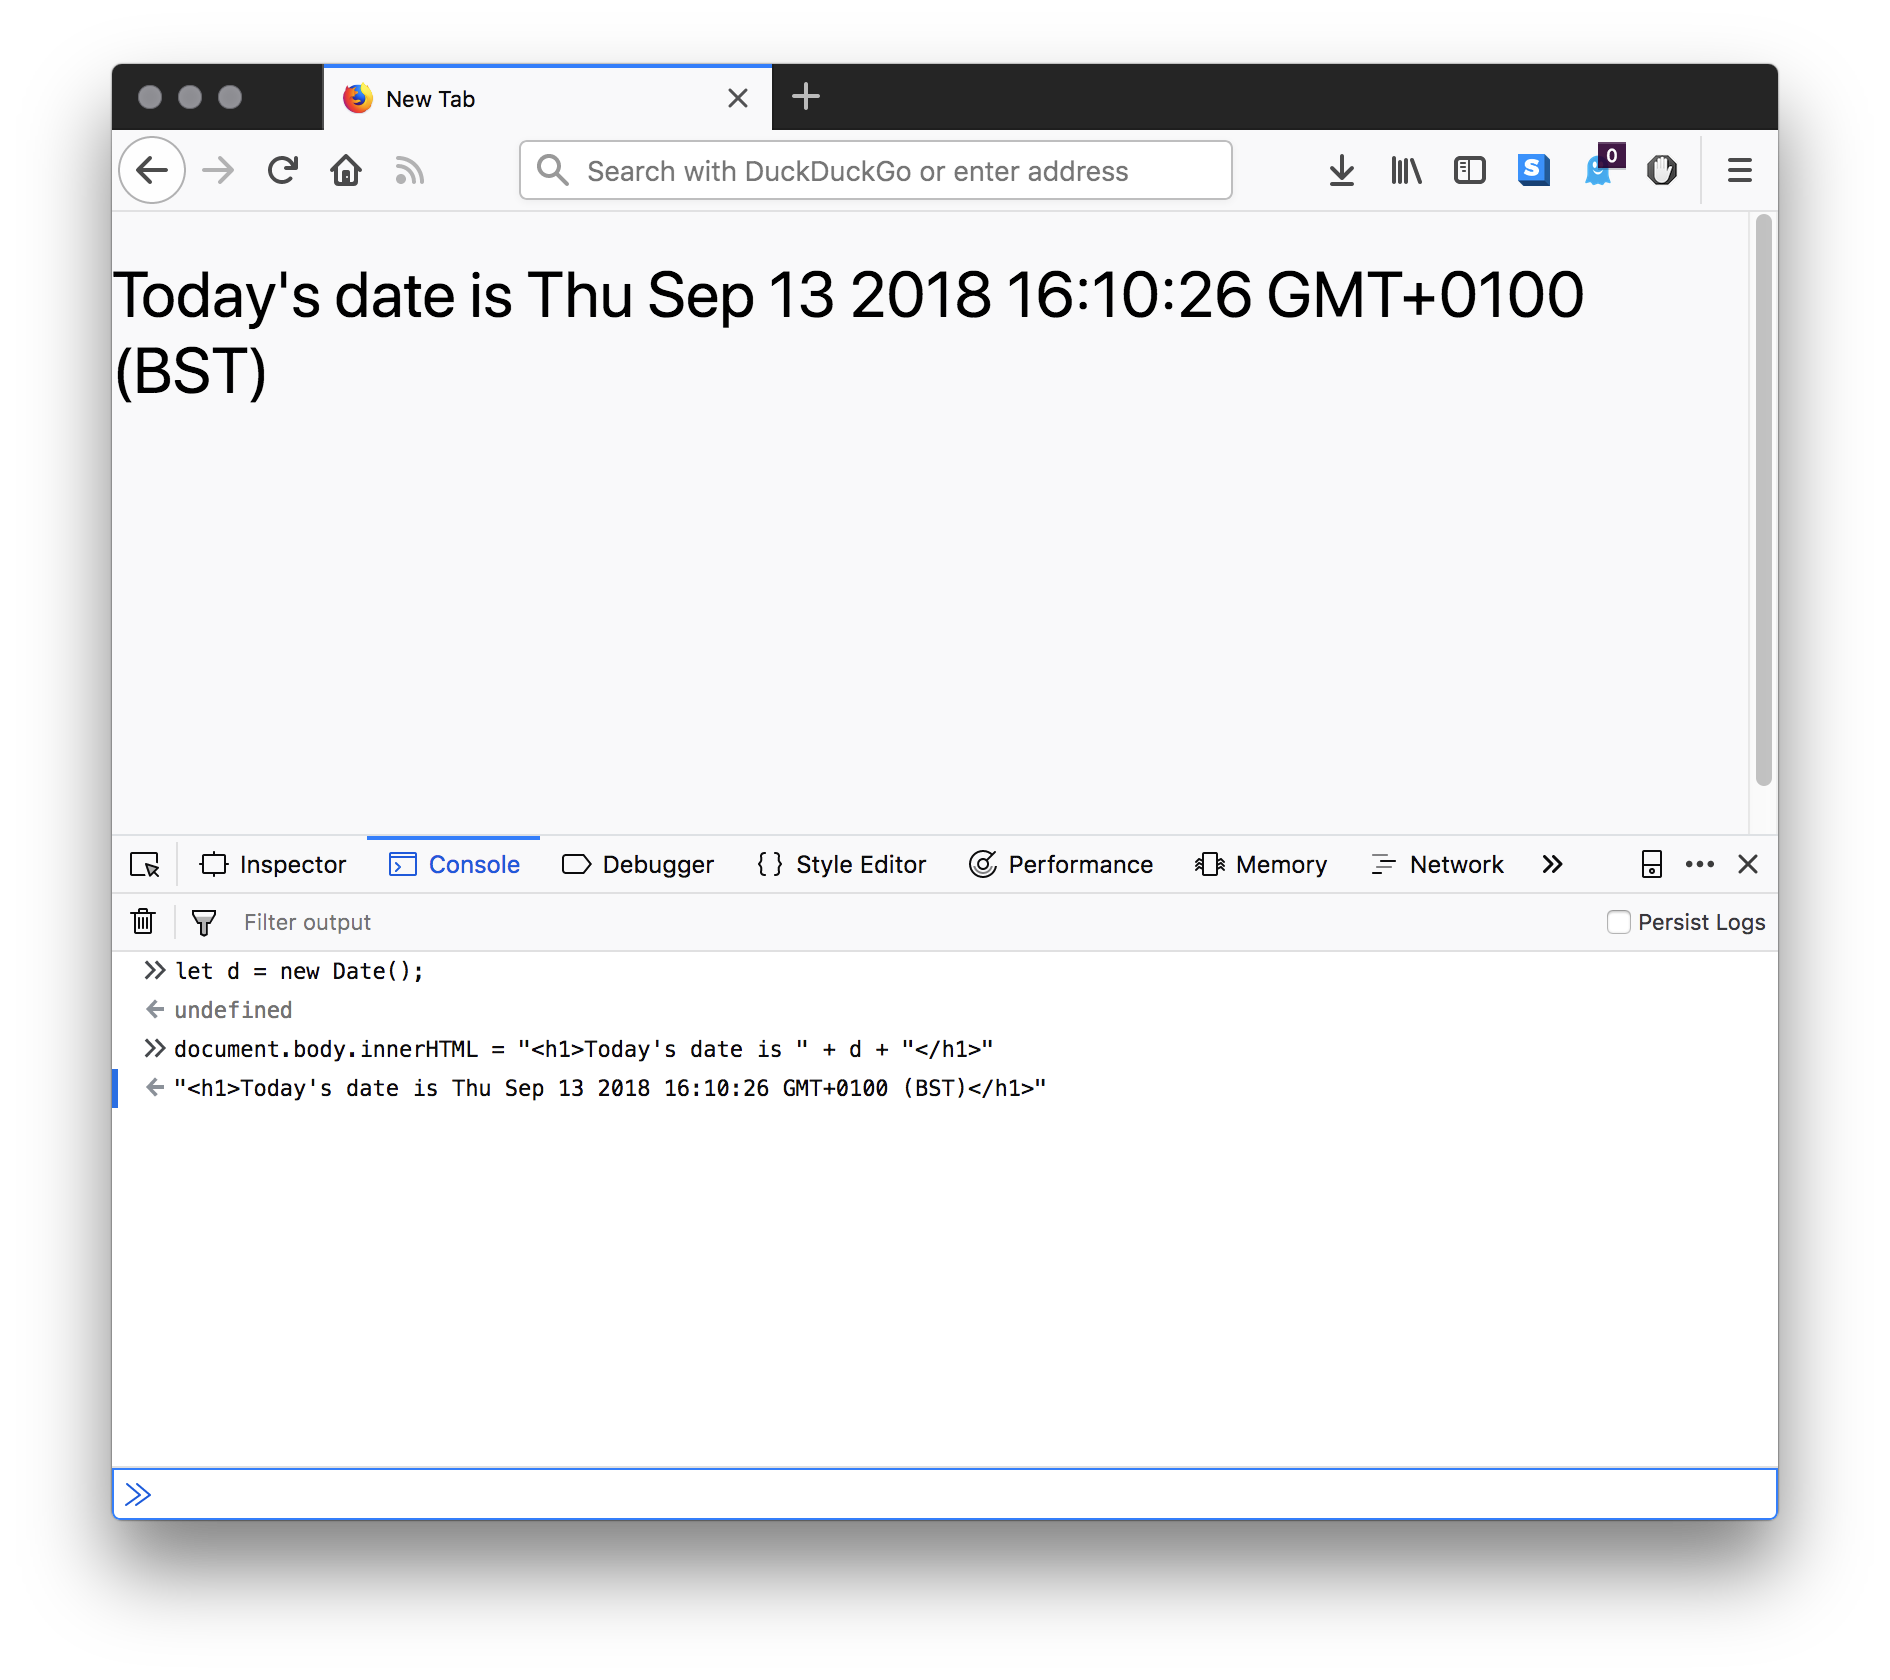
\includegraphics[width=0.8\textwidth]{figures/js-standard-functions}
\label{fig:js-standard-functions}
\caption{}
\end{figure}


\section{Construct A web Page}
\paragraph{} In this example we are going to construct a simple web page entirely from scratch using JS. First some variable, `p; to store a paragraph element, and `t' to store a text node that contains the content for the paragraph element. We then append our text, t, as a child of the paragraph, p and then replace the body of the document, the existing content, with our new paragraph node and its encapsulated text node child.

\begin{figure}[H]
\centering
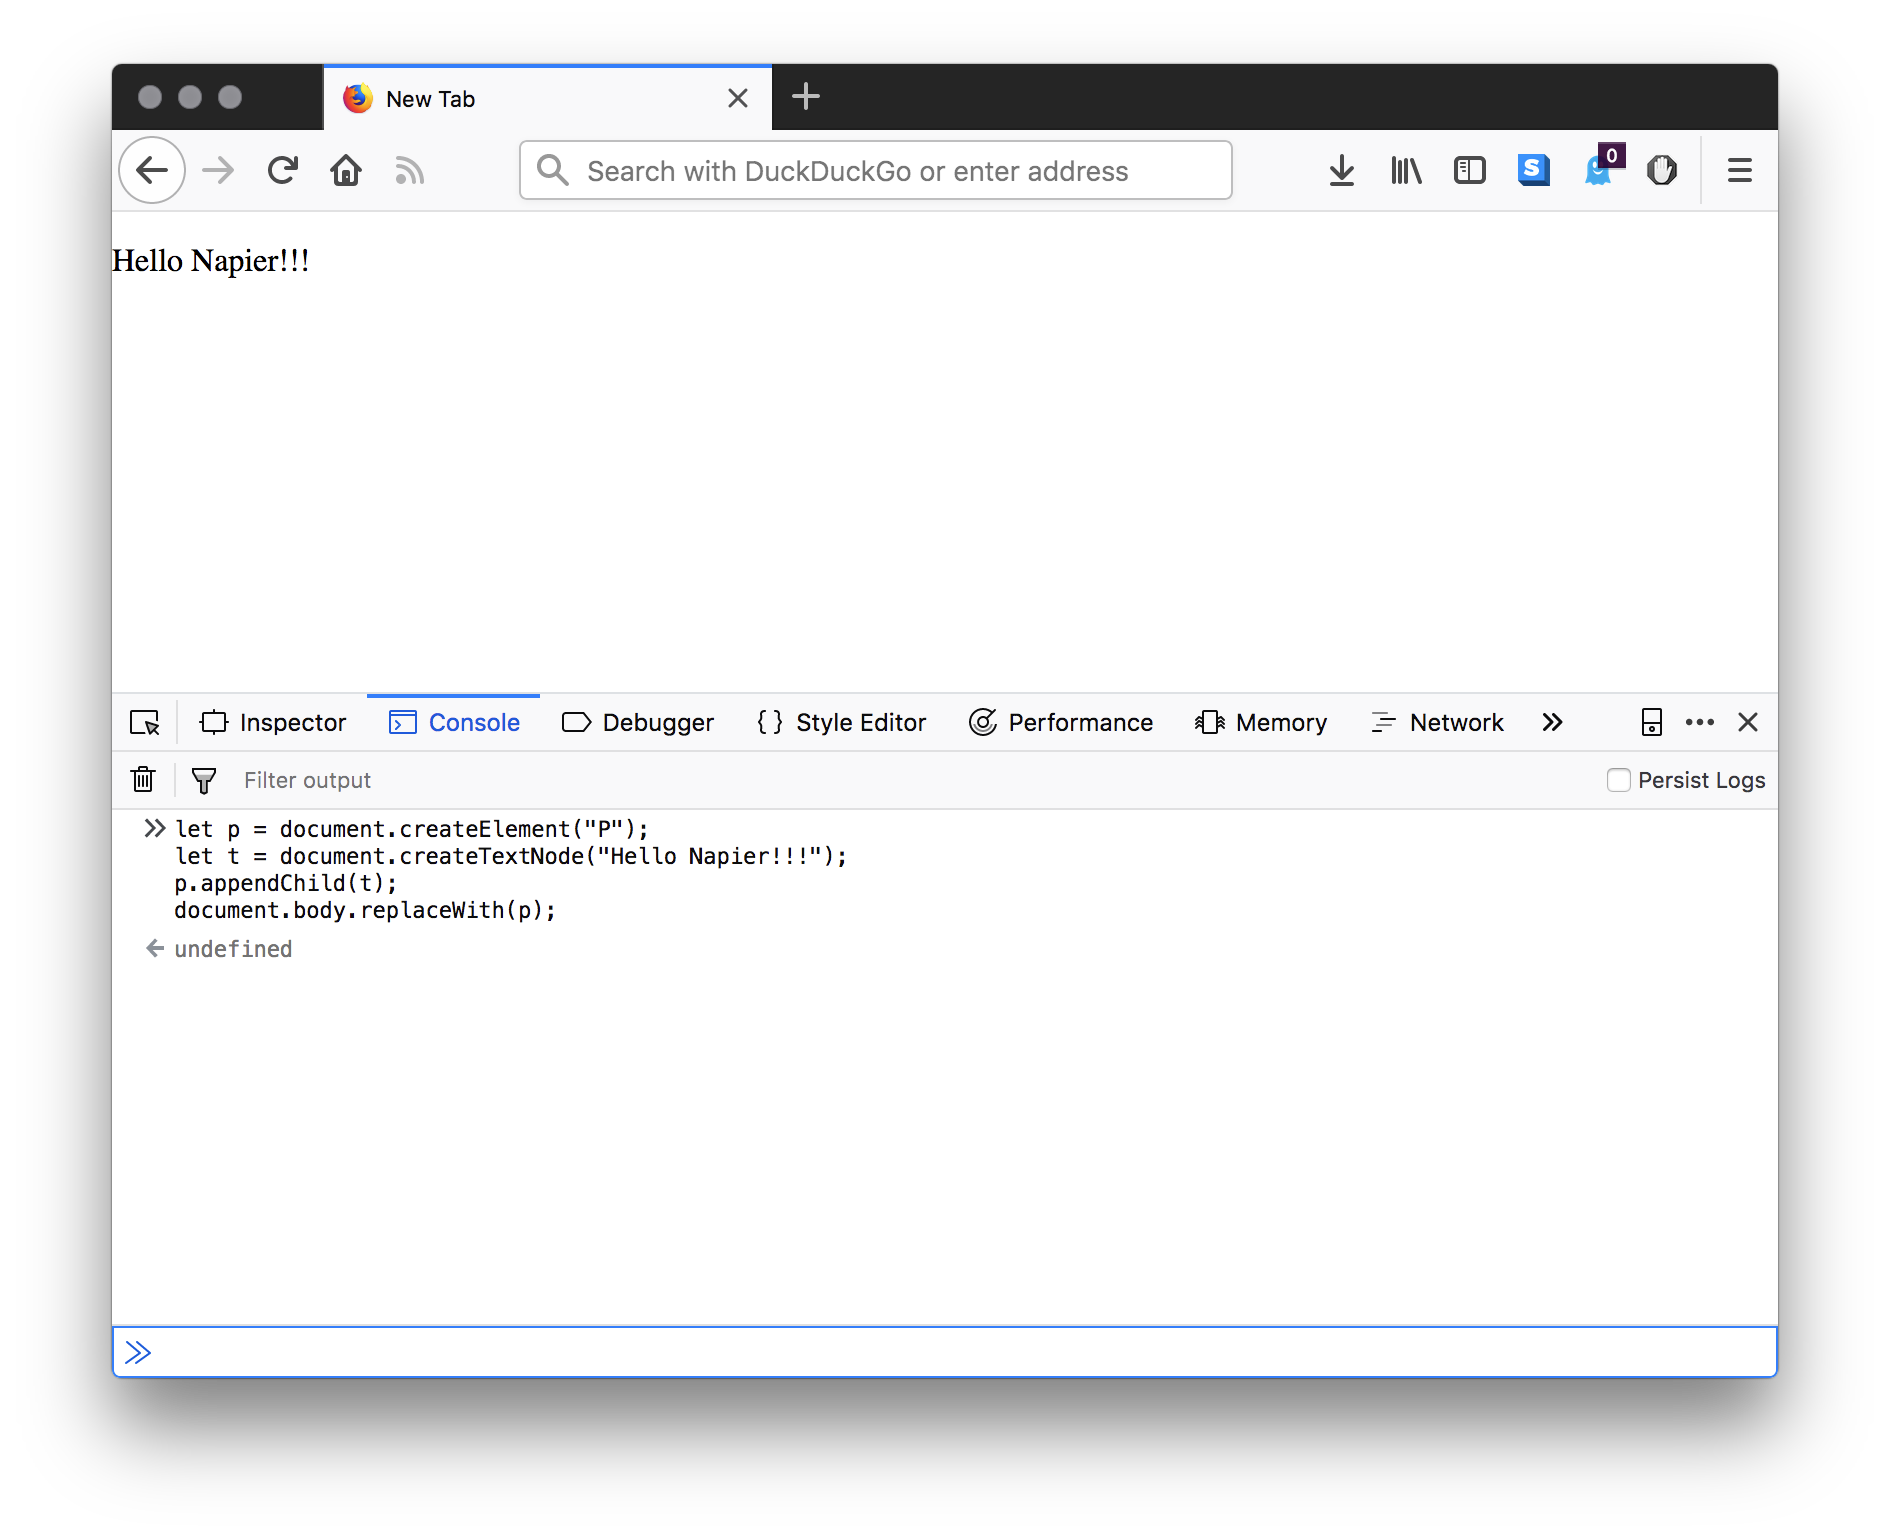
\includegraphics[width=0.8\textwidth]{figures/js-construct-page}
\label{fig:js-construct-page}
\caption{}
\end{figure}


\section{Graphics}
\paragraph{} This example is a very simple usage of the graphics API to draw a circle on a canvas element. The HTML canvas element is an HTML element that is designed to hold 2D and 3D graphics, as opposed to text which many HTML elements hold.
\paragraph{} We create a few variables in this example, the first being the canvas element, c, and the second being a variable for the drawing context which we set to 2D and then subsequently interact with to create our actual graphics. On our canvas we want to draw a circle. If we were using a pencil in the real world, then a circle would be a single pencil line. In the canvas context, this line is called a path, and we tell the canvas drawing context that we want a path to be drawn using an arc. Bear in mind that a circle is an arc that begins and ends in the same place and follows a constant angle. We specify how the stroke of the path should be drawn, because we don't actually have a pencil here so we need to say what we want the path to look like. We can alter the style of the stroke, but for now we'll accept the default. Finally we replace the existing document body with our new canvas which causes the page to be redrawn with our new canvas as the sole content containing our new circle.

\begin{figure}[H]
\centering
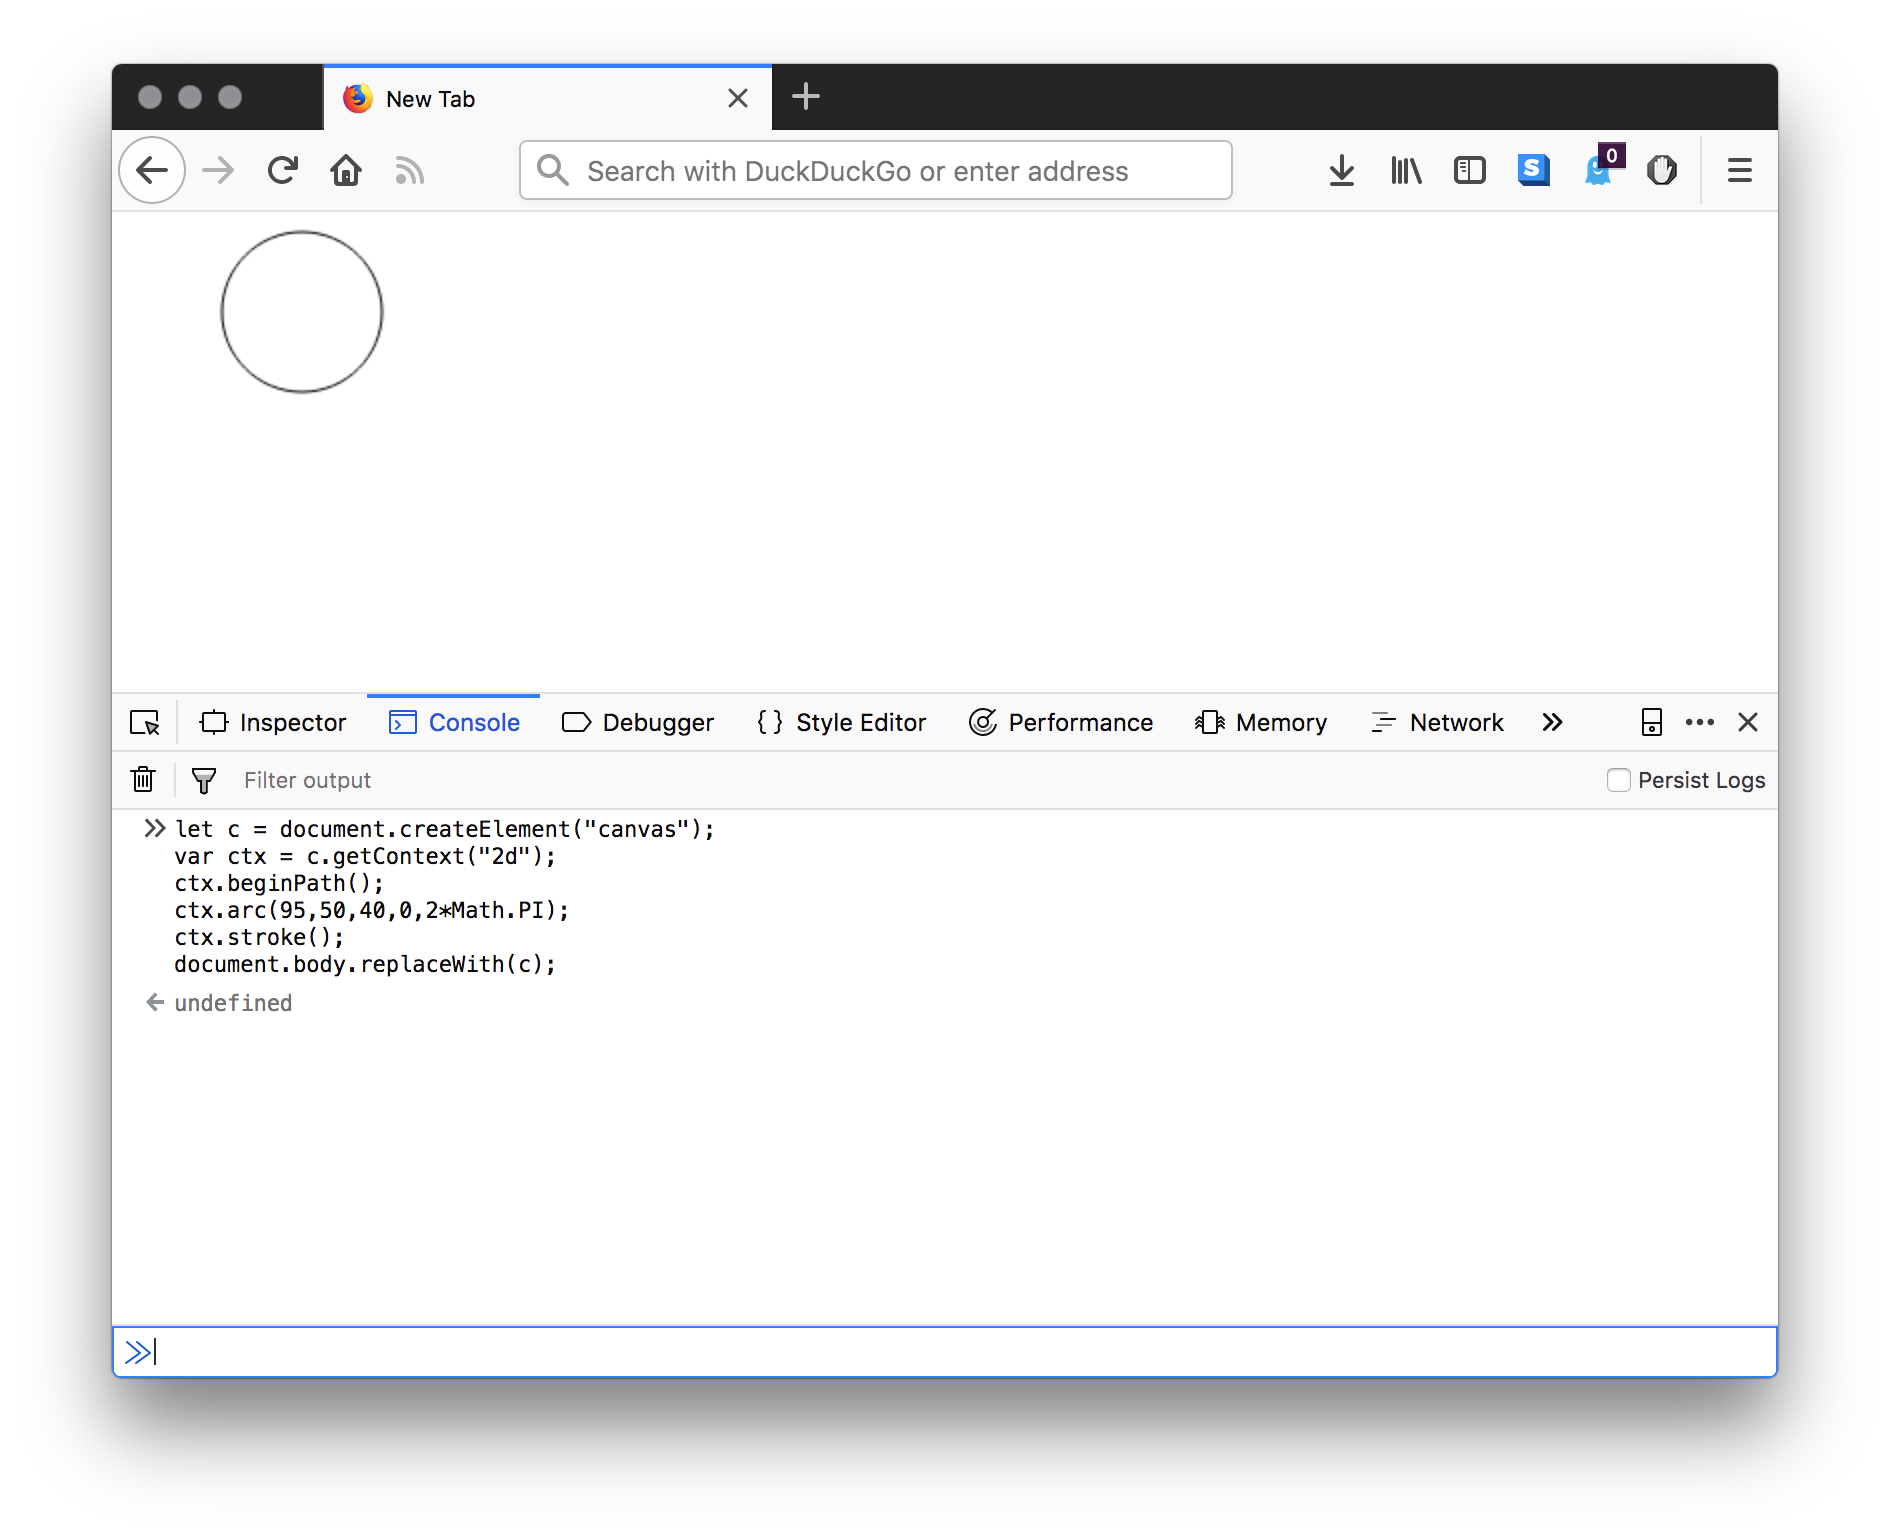
\includegraphics[width=0.8\textwidth]{figures/js-graphics}
\label{fig:js-graphics}
\caption{}
\end{figure}


\section{Sounds: Beeps}
\paragraph{} As well as graphics we can work with audio. In this example we create an audio context then build our sound from scratch. Sound is characterised by a waveform of a given frequency and that waveform is created by an oscillator. So we create our context variable and use it to retrieve a handle to the browser window's audio context. We then create a variable to hold our oscillator and set the waveform type, or shape, to "sine" for a sine wave and the frequency to 440Hz. The oscillator is then connected to the audio context and set to start which causes it to play and, as a result, make a noise.


\begin{figure}[H]
\centering
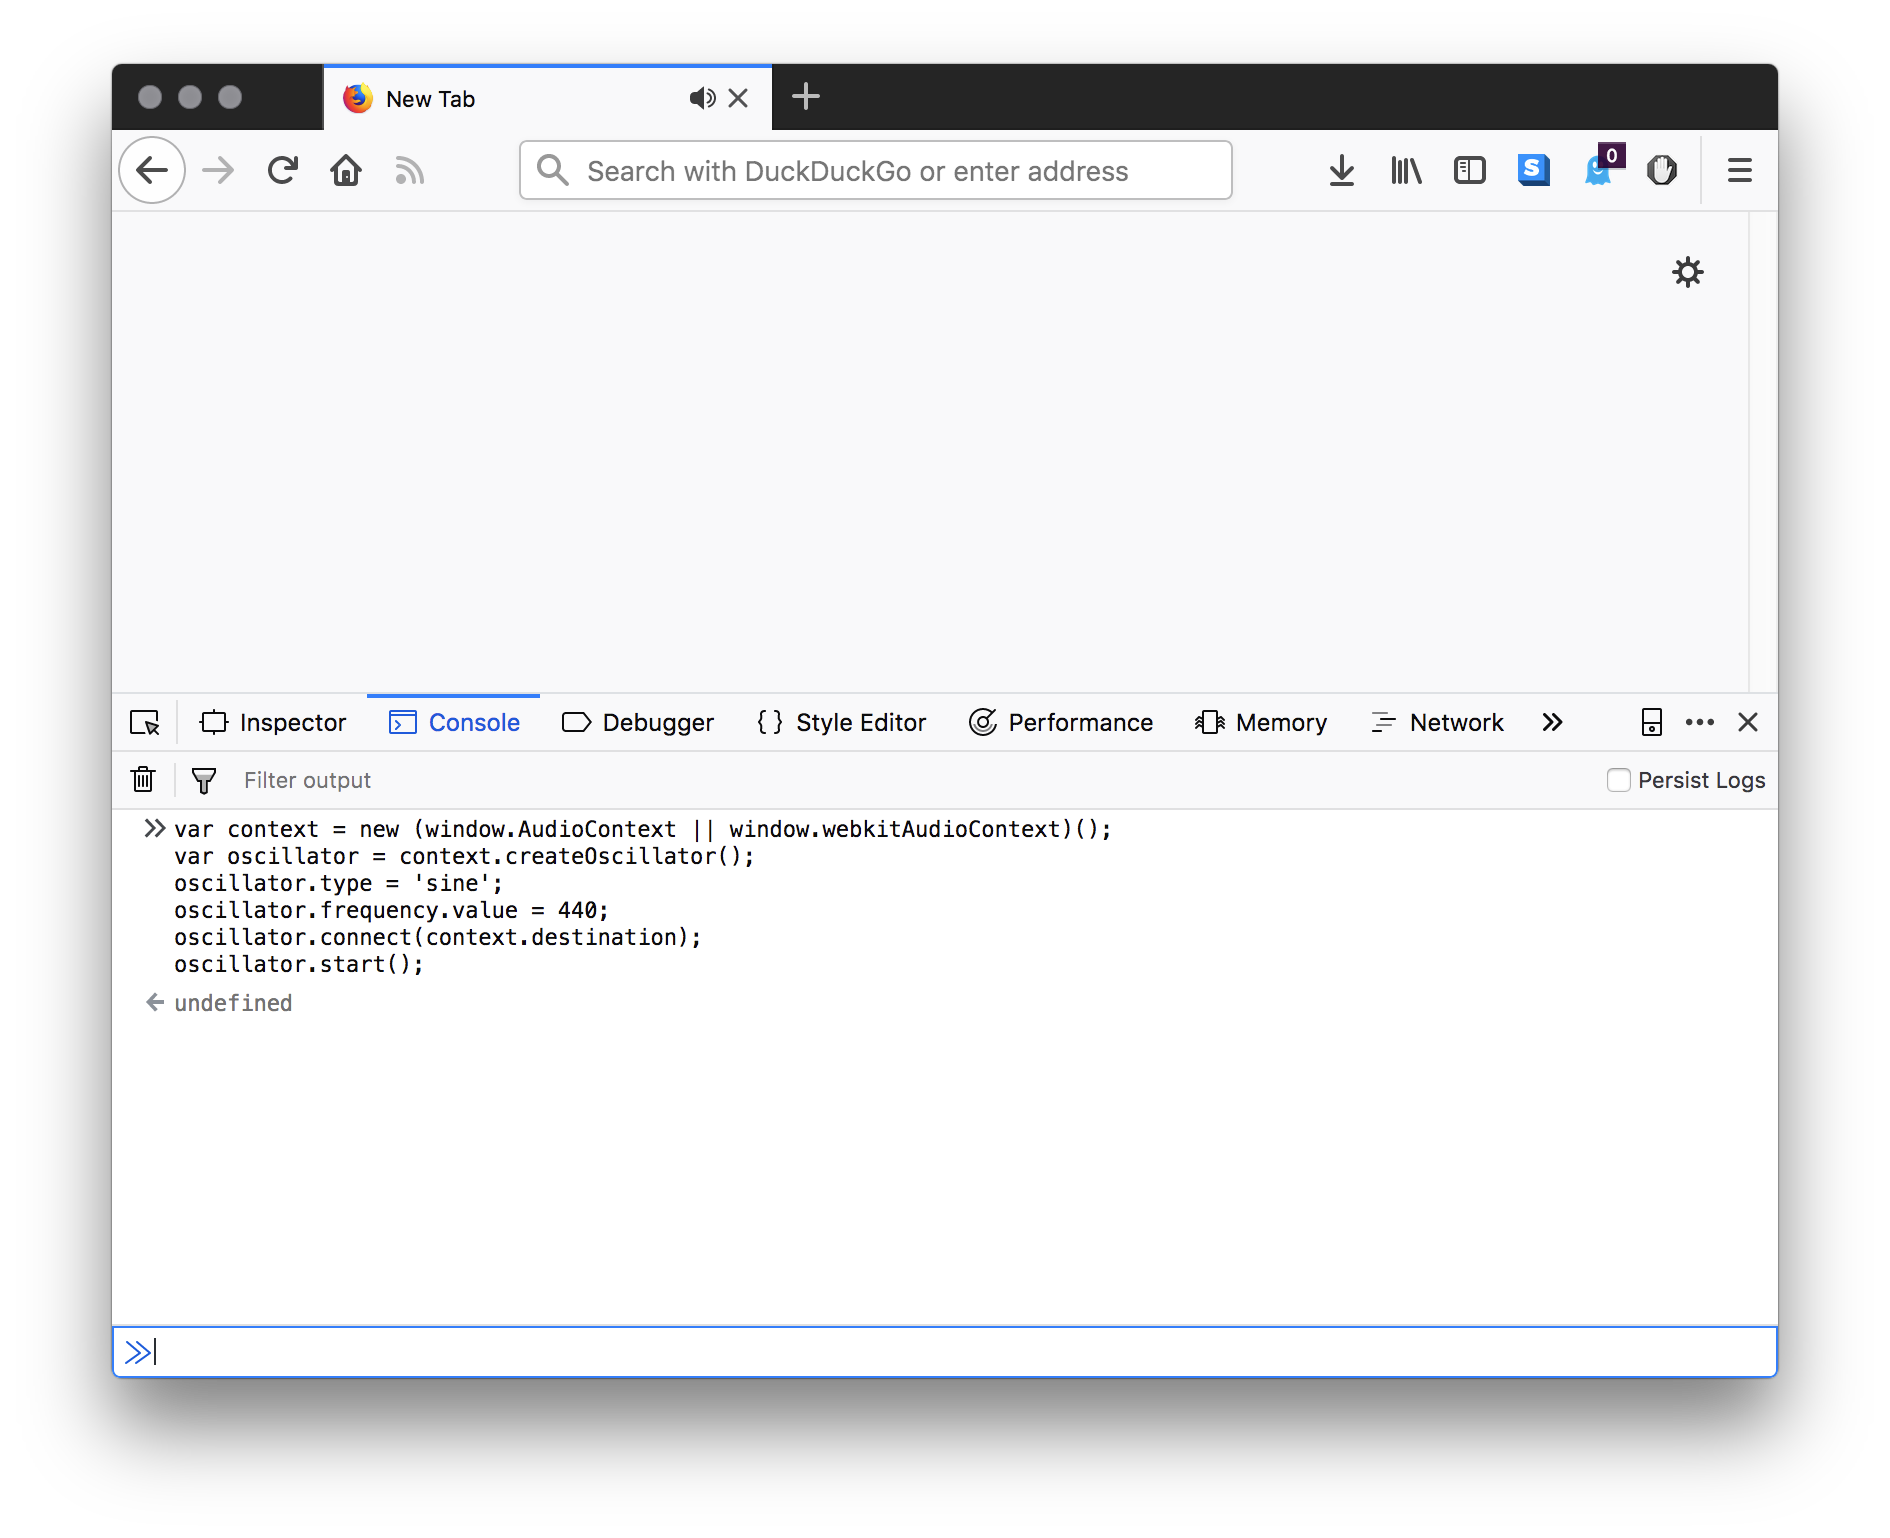
\includegraphics[width=0.8\textwidth]{figures/js-sounds}
\label{fig:js-sounds}
\caption{}
\end{figure}


\section{Sound: ChipTunes}

\paragraph{} We can go further than mere beeps though. So in this example we create a slightly more complex example that shows a way to play a variety of different sounds for different lengths of time. If we play different sounds in sequence, then we have a rudimentary tune. This is how we can build music from first principles.

\begin{figure}[H]
\centering
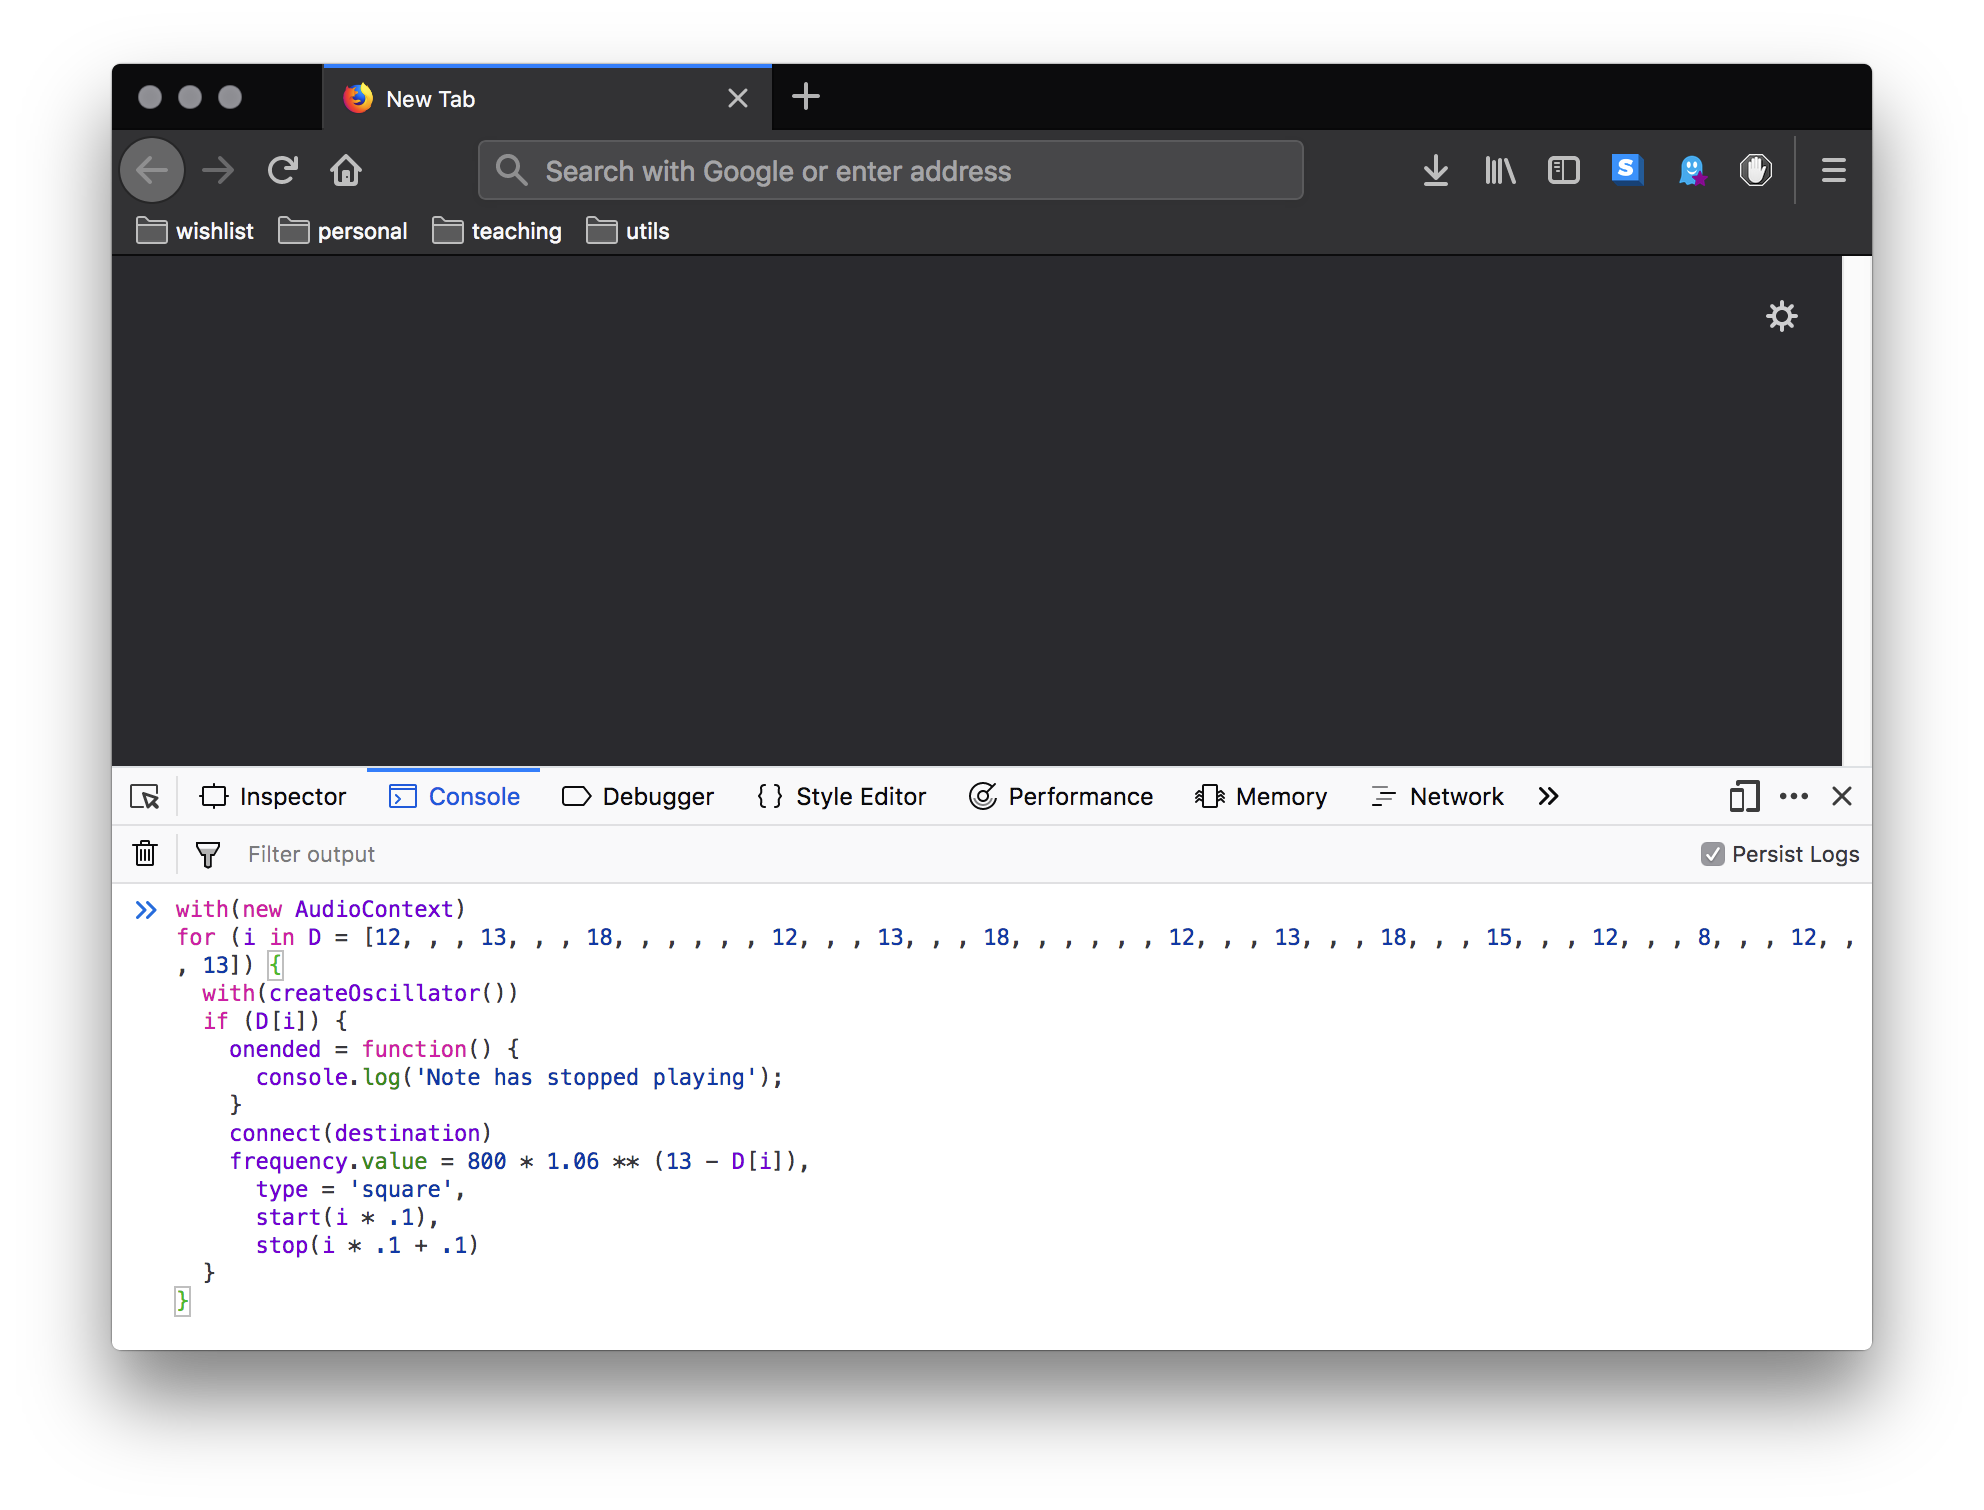
\includegraphics[width=0.8\textwidth]{figures/js-chiptunes}
\label{fig:js-chiptunes}
\caption{}
\end{figure}


\section{Sound: Theremin}
\paragraph{} In this final example we create an audio context and oscillator as before. However this time we've also added an event listener to the document which accesses the mouse pointer location. This is connected to the oscillator and we use the location of the mouse pointer to alter the oscillators frequency. In essence, we've created a version of an esoteric musical instrument called a Theremin. This shows one way that we can use user interaction to affect the audio that is played by the browser.

\begin{figure}[H]
\centering
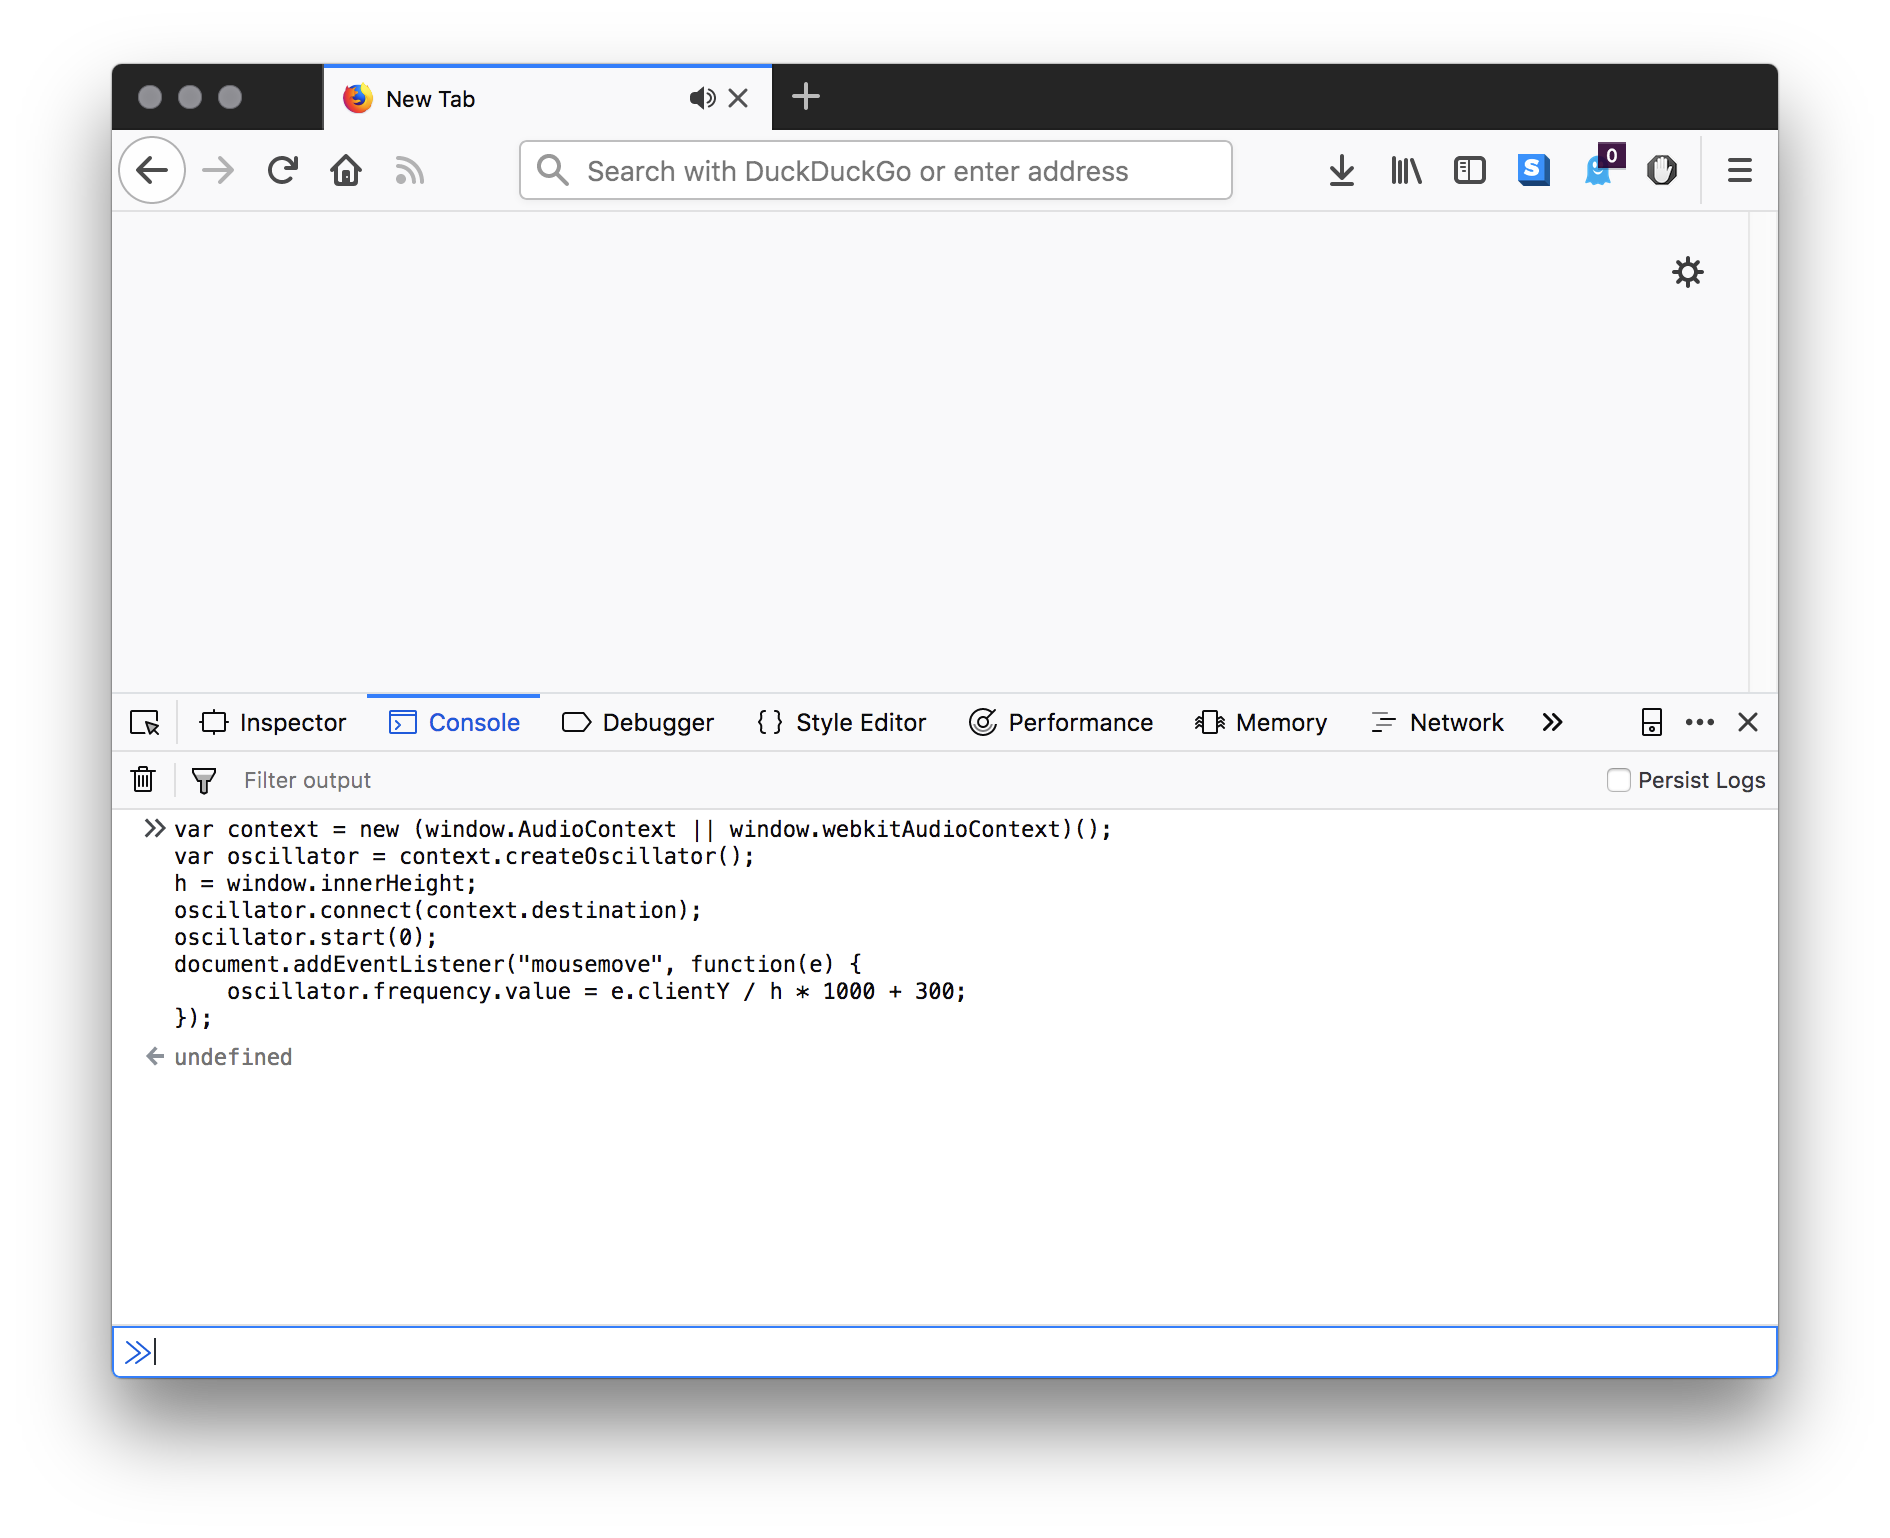
\includegraphics[width=0.8\textwidth]{figures/js-theremin}
\label{fig:js-theremin}
\caption{}
\end{figure}


\section{JS as a Language}
\paragraph{} Having tried out some JS and seen a little of what JS can do in the browser, we can, with the benefit of hindsight and some experience, now look at the language in a little more detail. Remember though that this overview of the language assumes that you can already program in some language. It is not aimed at teaching you to program but at helping you to add JS as a new language to your toolbox which should already contain at least one other language. If you already know some C-syntax style language like C, C++, C\#, Java, Python, etc. then you will find that there is quite a bit of syntactic overlap. Obviously the detail can be very different, but the basic programming approach is similar and generally knowledge from one of these languages can be quite applicable to JS.
\paragraph{} IMPORTANT: If you want to become a good programmer in any language then you need to practise. Reading code or documentation is much less useful than actually writing code and solving problems.
\paragraph{} Let's look at JavaScript as a standalone language. By this we mean that we want to consider such things as:

\begin{itemize}
\item keywords, commenting, variables, primitive datatypes, native objects, and operators
\item Examine control structures (if-else, conditional, switch) and looping
\item Functions, Objects, and Exception handling
\item JavaScript object serialisation using JSON
\end{itemize}

\section{Case, Whitespace, and Statement Separators}
\paragraph{} JS is case sensitive. As with all programming we have to be precise so you can't alternate between upper and lower case as they don't always mean the same thing. It is best to develop a habit for using case then stick to it. I nearly always use lowercase (and also choose snake\_case rather than camelCase when naming things).
\paragraph{} Spaces, tabs, and newlines outside of strings are whitespaces but JS is not whitespace sensitive, unlike, say, Python. This is generally not a problem so you should choose a way to use whitespace then be consistent in laying out your code.
\paragraph{} Semicolons are used to separate statements. However, like many web technologies, you can leave them out of your code and the JS engine will automatically insert them for you. However, in certain circumstances code can be ambiguous and the engine can make an incorrect choice of where to insert a semicolon. This can interfere with whitespace handling and cause valid code to be incorrectly parsed resulting in an error or incorrect functionality. As a result it is generally good practice to end statements with a semicolon.


\section{JS Keywords}
\paragraph{} JS has a number of keywords that can be organised into four groups according to whether they are core JS keywords, built-in keywords, DOM and Window object related keywords, and event related keywords. You should avoid any of the following when naming your own variables, function names, or labels but obviously use them when you want to use these keywords as intended by the JS language.

\begin{description}
\item [JavaScript keywords] abstract, arguments, await*, boolean, break, byte, case, catch, char, class*, const, continue, debugger, default, delete, do, double, else, enum*, eval, export*, extends*, false, final, finally, float, for, function, goto, if, implements, import*, in, instanceof, int, interface, let*, long, native, new, null, package, private, protected, public, return, short, static, super*, switch, synchronized, this, throw, throws, transient, true, try, typeof, var, void, volatile, while, with, yield
\item [Built-in Objects, Properties, \& Methods]  Array, Date, eval, function, hasOwnProperty, Infinity, isFinite, isNaN, isPrototypeOf, length, Math, NaN, name, Number, Object, prototype, String, toString, undefined, valueOf
\item [HTML \& Window objects \& properties] alert, all, anchor, anchors, area, assign, blur, button, checkbox, clearInterval, clearTimeout, clientInformation, close, closed, confirm, constructor, crypto, decodeURI, decodeURIComponent, defaultStatus, document, element, elements, embed, embeds, encodeURI, encodeURIComponent, escape, event, fileUpload, focus, form, forms, frame, innerHeight, innerWidth, layer, layers, link, location, mimeTypes, navigate, navigator, frames, frameRate, hidden, history, image, images, offscreenBuffering, open, opener, option, outerHeight, outerWidth, packages, pageXOffset, pageYOffset, parent, parseFloat, parseInt, password, pkcs11, plugin, prompt, propertyIsEnum, radio, reset, screenX, screenY, scroll, secure, select, self, setInterval, setTimeout, status, submit, taint, text, textarea, top, unescape, untaint, window
\item [HTML Event Handlers] onblur, onclick, onerror, onfocus, onkeydown, onkeypress, onkeyup, onmouseover, onload, onmouseup, onmousedown, onsubmit
\end{description}

\section{Comments}

\paragraph{} There are two basic ways to insert your own comments into your JS. Like so:

\begin{lstlisting}
// A short, one line comment
\end{lstlisting}

\paragraph{} or like so:

\begin{lstlisting}
/* a longer, multi-line 
comment about something 
that must be important */
\end{lstlisting}

\paragraph{} Note that:

\begin{lstlisting}
/* Comments /* cannot be nested */ as this is a syntax error */
\end{lstlisting}


\section{Variables}
\paragraph{} Variables can be declared in three ways:

\begin{itemize}
\item Block level variables using the let keyword
\item Function level variables using the var or const keywords
\end{itemize}

\paragraph{} Variables in JS don’t have a type attached. This means that any value can be stored in any variable. This is different to other languages, like C for instance, which require a type to be specified for every variable.

\paragraph{} A variables value is undefined until it is initialised, e.g. 

\begin{lstlisting}
	var a = 203
\end{lstlisting}

\paragraph{} A variable declared anywhere inside a function will resolve to that variable when its name is used within the function but variables declared outside a function are global. If you try to use a variable but it can't be found by the JS engine then a ReferenceError exception will happen.


\section{Primitive Datatypes}
\paragraph{} Although we don't have to declare a variables datatype, that doesn't mean that they don't exist in JS. There are a number of primitive datatypes available, these include Undefined, Null, Number, String, Boolean, and Symbol.
\paragraph{} Let's consider each in turn:

\begin{description}
\item [Undefined] This is assigned to all uninitialised variables and returned where checking for object properties that don’t exist.
\item [Null] This is used when a variable has been declared but the value is empty.
\item [Numbers] These are IEEE754 standard doubles. They are floating point numbers which can be rounded to whole numbers using the toFixed() function. The accuracy of primitive JS numbers is 16 significant digits.
\item [Strings] These are handled as a sequence of characters enclosed in double quotes. Individual letters in a string can be accessed using the charAt() function. Strings can be compared using '=='.
\item [Boolean] Standard boolean binary values of true and false are available to be used for comparisons.
\item [Symbol] This is new to JS as of the ECMAScript 6 specification and are used to create a unique and immutable identifier.
\end{description}



\section{Native Objects}
\paragraph{} JS includes a range of useful native objects including Arrays, Dates, Errors, Math, Regular Expressions, and Functions.
\paragraph{} Let's briefly consider each in turn:

\begin{description}
\item [Arrays] These are objects that represent lists of values. Arrays are indexed by keys which are numeric and use zero based indexing. Arrays can be multi-dimensional so they can be used for matrices of various dimensions.
\item [Date] This is an object that stores a signed millisecond count from zero. Zero represents the following date: 1970-01-01 00:00:00 UT and everything else is an offset from that zero point. The date object supports various methods to access fields of the date object.
\item [Error] An object that can be used to create custom error messages.
\item [Math] An object that stores various mathematics related constants such as values for E, the natural Log, Pi, \&c. It also support various functions like max(), min(), and random() amongst others.
\item [Regular Expressions] An object that is used to store text patterns and extremely useful when needing to find instances of some search pattern within another body of text.
\item [Function] An object that is constructed using the Function constructor and used to collect statements into reusable groups. An awful lot of JS programming comprises writing functions.
\end{description}



\section{Operators}
\paragraph{} There is a full complement of the standard operators that you should recognise from other programming languages. These include the following:

\begin{description}
\item [Arithmetic] +, -, *, /, \%
\item [Unary] + (string to number), - (reverse sign), ++, —
\item [Assignment] =, +=, -+, *=, /=, \%= 
\item [Destructuring assignment] [a, b, c] = [3, 4, 5];
\item [Logical] !, $\vert\vert$, \&\&
\item [String] =, +, +=
\end{description}

\paragraph{} NB. There are also bitwise operators and assignments as well as a ternary conditional.



\section{Control Structures}
\paragraph{} We need control structure to enable us to affect the flow of our programs, letting us check conditions and branch to different paths of execution. The standard control structures include the if/else structure, the conditional operator, and the switch statement. Again, these should all be familiar from languages that you've already experienced and all work in a fairly similar way.

\subsection{if/else}

\begin{lstlisting}
if (expr) {
	//statements;
} else if (expr2) {
  	//statements;
} else {
  	//statements;
}
\end{lstlisting}

\subsection{Conditional Operator}

\begin{lstlisting}
result = condition ? expression : alternative
\end{lstlisting}

\subsection{Switch Statement}
\begin{lstlisting}
switch (expr) {
  	case SOMEVALUE:
   		// statements;
		break;
  	case ANOTHERVALUE:
   		// statements;
   		break;
  	default:
   		// statements;
   	break;
 }
\end{lstlisting}



\section{Looping}
\paragraph{} When we need to do something more than once, a standard strategy is to loop over the statements however many times are required. JS supports the standard approaches to looping that we should recognise from other C style languages and syntaxes. These include:

\subsection{For Loop}

\begin{lstlisting}
for (initial; condition; loop statement) {
  	/*
   	statements will be executed every time the for{} loop cycles, while the
   	condition is satisfied
  	*/
 }
\end{lstlisting}

\subsection{For In Loop}

\begin{lstlisting}
for (var property_name in some_object) {
  	// statements using some_object[property_name];
}
\end{lstlisting}

\subsection{While Loop}

\begin{lstlisting}
while (condition) {
  	statement1;
  	statement2;
  	statement3;
  	...
}
\end{lstlisting}

\subsection{Do/While Loop}
\begin{lstlisting}
do {
  	statement1;
  	statement2;
  	statement3;
  	...
} while (condition);
\end{lstlisting}


\section{Functions}
\paragraph{} Functions are at the core of JS programming. There are various ways to declare (create) functions. For example:

\paragraph{} Using the function keyword to define a function:

\begin{lstlisting}
function add(x,y) { return x + y; };
\end{lstlisting}

\paragraph{} Using the function keyword to define a function and assigning it to a variable:

\begin{lstlisting}
var add = function(x,y) { return x + y; };
\end{lstlisting}

\paragraph{} Creating a new function and assigning it to a variable using the Function() function

\begin{lstlisting}
var add = new Function(‘x’, ‘y’, ‘return x + y’);
\end{lstlisting}



\section{Objects}
\paragraph{} JS supports object orientation using a form of Object Oriented Programming (OOP) that uses prototype-based inheritance. We can create objects and assign data and method to them in at least four different ways but this is mostly syntactic sugar. The following is probably the easiest way to create an object in JS, by just using an object literal. An object literal is an instance of the JS global Object() object type. Let's see it in action:

\begin{lstlisting}
var cow = {
  	colour:'brown',
  	commonQuestion:'What now?',
  	moo:function(){ console.log('moo'); },
  	feet:4,
  	accordingToLarson:'will take over the world'
};
\end{lstlisting}

\paragraph{} This gives you an object called cow that you can interact with, e.g. cow.moo(). Another way to do this is to create a new object then set its parameters, like so:

\begin{lstlisting}
var cow = new Object();
cow.colour = 'brown';
cow.commonQuestion = 'What now?';
cow.moo = function(){ console.log('moo'); }
cow.feet = 4;
cow.accordingToLarson = 'will take over the world';
\end{lstlisting}

\paragraph{} We can also use a constructor function to simplify things, especially if we want to instantiate multiple different objects, e.g.

\begin{lstlisting}
function Cow(colour, commonQuestion, feet, accordingToLarson) {
	this.colour = colour;
	this.commonQuestion = commonQuestion;
	this.feet = feet
	this.accordingToLarson = accordingToLarson;
	this.moo = function(){ console.log('moo'); };
}

var cow = new Cow("brown", "what now?", 4, "will take over the world");
\end{lstlisting}

\paragraph{} Note that with this approach it doesn't let you pass the functions into the constructor, they need to be predefined in the constructor function, e.g. the moo() function. In more recent versions of JS, based upon the ECMASCRIPT 6 specification you can also use the new class syntax that is similar to other languages.

\begin{lstlisting}
class Cow {
	constructor(colour, commonQuestion, feet, accordingToLarson) {
		this.colour = colour;
		this.commonQuestion = commonQuestion;
		this.feet = feet
		this.accordingToLarson = accordingToLarson;
		this.moo = function(){ console.log('moo'); };
	}
}

var cow = new Cow("brown", "what now?", 4, "will take over the world");
\end{lstlisting}

\paragraph{} The only real difference between this and the previous example is the use of the class and constructor syntax. Yet another way to create objects is with the Object.create() method, e.g.

\begin{lstlisting}
var cow = {
  	colour:'brown',
  	commonQuestion:'What now?',
  	moo:function(){ console.log('moo'); },
  	feet:4,
  	accordingToLarson:'will take over the world'
};

var cow2 = Object.create(cow);
\end{lstlisting}

\paragraph{} Which creates a new object, cow2, whose parameters you can then update to differentiate it from the other cow object literal.



\section{Exception Handling}
\paragraph{} Your programs are unlikely to be perfect, and even if they are, unexpected circumstances can still occur. To help deal with these circumstances we can use exception handling.
We can handle run time errors by:

\begin{enumerate}
\item Trying to execute the statements
\item Catching any thrown exceptions
\item Finally cleaning things up.
\end{enumerate}

\paragraph{} e.g.

\begin{lstlisting}
try {
  	// Statements in which exceptions might be thrown
} catch(errorValue) {
  	// Statements that execute in the event of an exception
} finally {
  	// Statements that execute afterward either way
}
\end{lstlisting}

\section{Best Practices}
\paragraph{} Just a few tips and best practices for starting off your JS programming style. Some of these are debatable but thinking about them will make you into a better web developer.

\begin{itemize}
\item Call things by their name — easy, short and readable variable and function names
\item Avoid globals
\item Stick to a strict coding style
\item Comment as much as needed but not more
\item Avoid mixing with other technologies
\item Use shortcut notation when it makes sense
\item Modularise — one function per task
\item Enhance progressively
\item Allow for configuration and translation
\item Avoid heavy nesting
\item Optimize loops
\item Keep DOM access to a minimum
\item Don’t yield to browser whims
\item Don’t trust any data
\item Add functionality with JavaScript, don’t create too much content
\item Build on the shoulders of giants
\item Development code is not live code
\end{itemize}

\paragraph{} The W3C keeps an annotated list\footnote{\url{https://www.w3.org/wiki/JavaScript_best_practices}} of best practices that is worth keeping an eye on as you develop your JS skills


\section{Summary}
\paragraph{} In thischapter we've started to explore the JavaScript language. We should now understand the role that JavaScript plays amongst the other core web technologies and have some idea of how JavaScript interacts with HTML, CSS, and the Browser. We've also surveyed the core JavaScript syntax so we are now ready to start exploiting it within our Web pages.
